\documentclass[thesis.tex]{subfiles}

\DeclareGraphicsRule{*}{mps}{*}{}
 
\begin{document}
\chapter{Theory and Motivation}
\label{ch1}

\section{The Standard Model}
The Standard Model (SM) of particle physics is a well-tested and successful theory that describes the known elementary particles and their interactions. 
It is built within a framework known as Quantum Field Theory (QFT), which provides the mathematical tools to describe the subatomic particles using theories that are consistent with both quantum mechanics and special relativity. 
In QFT, particles are represented by excitations of quantum fields. 
The dynamics and interactions of the particles are governed by the Lagrangian density $\mathcal{L}$.

Throughout this thesis we use the natural units, defined by:
\begin{equation}
	c = \hbar = 1,
\end{equation}
where $\hbar$ is the reduced Planck constant and c is the speed of light. 
Using this convention, mass, energy, and momentum can be expressed with the same unit: eV.
For heavy particles, MeV ($=10^3$ eV) and GeV ($=10^6$ eV) are used.

The SM consists of a set of matter particles and force carriers, as well as the Higgs boson which gives mass to all fundamental particles. 
Table \ref{tab:SM} summarises the SM particles and their properties.
These particles are classified into two groups: fermions with half-integer spin, and bosons with integer spin.
Fermions are further grouped into three generations, with masses increasing from one generation to the next. 

\begin{table}[h]
\centering
\caption{Summary of the particle content of the Standard Model, along with their properties.}
\resizebox{\textwidth}{!}{
\begin{tabular}{ |c|c|c|c|c|c|c|c|c|c| }
	\hline
	\multicolumn{10}{ |c| }{Standard Model particles} \\
	\hline \hline
	\multicolumn{10}{ |c| }{Fermion: spin 1$/$2 } \\
	\hline
		& \multicolumn{3}{c}{1st generation} & \multicolumn{3}{ |c| }{2nd generation} & \multicolumn{3}{ |c| }{3rd generation} \\
	\cline{2-10}
						& particle 			& charge 			& mass 			& particle 			& charge 			& mass			& particle 			& charge 			& mass \\
	\hline
	\multirow{2}{*}{Lepton} 	& e            		& $\pm$ 1    		& 0.511 MeV 			& $\mu$			& $\pm$ 1 		& 0.105 GeV 				& $\tau$ 			& $\pm$ 1 		& 1.7768 GeV \\
	\cline{2-10}
	                                    	&$\nu_e$  		&  0              		& $<$ 2.2 eV    &$\nu_\mu$  	&  0              		& $<$ 1.7 MeV          &$\nu_\tau$  		&  0             		&  $<$ 15.5 MeV    \\
	\hline
	\multirow{2}{*}{Quark}  	&  u           		&  $\pm 2/3$		& 2.4 MeV				 & c 				& $\pm 2/3$		& 1.275 GeV 				& t   				& $\pm 2/3$		& 172.44 GeV  \\
	\cline{2-10}
					    	& d           			&  $\mp 1/3$     	& 4.8 MeV 				 & s				&  $\mp 1/3$ 		 & 95 MeV				& b   				&  $\mp 1/3$ 		& 4.18 GeV \\ 
	\hline \hline
	\multicolumn{10}{ |c| }{Gauge Boson: spin 1 } \\
	\hline
	Partile  				&  \multicolumn{3}{c|}{Interaction}  		&   \multicolumn{3}{c|}{ Charge }		& \multicolumn{3}{c|}{ Mass (GeV) } 	 \\
	 \hline
	 $\gamma$ 			&  \multicolumn{3}{c|}{EM}  			&  \multicolumn{3}{c|}{ 0 }  			&   \multicolumn{3}{c|}{ 0 } \\
	 \hline
	 W 					&  \multicolumn{3}{c|}{Weak}  			&  \multicolumn{3}{c|}{ $\pm$ 1 }  		&   \multicolumn{3}{c|}{ 80.39 } \\
	 \hline
	 Z 					&  \multicolumn{3}{c|}{Weak}  			&  \multicolumn{3}{c|}{ 0 }  			&   \multicolumn{3}{c|}{ 91.19 } \\
	 \hline
	 g 					&  \multicolumn{3}{c|}{Strong}  			&  \multicolumn{3}{c|}{ 0 }  			&   \multicolumn{3}{c|}{ 0 } \\
	 \hline \hline
	 \multicolumn{10}{ |c| }{Higgs Boson: spin 0 } \\
	 \hline
	 H 					&  \multicolumn{3}{c|}{-}           			&   \multicolumn{3}{c|}{ 0 }  			&   \multicolumn{3}{c|}{ 125.09 } \\
	 \hline
	                                     
\end{tabular}
}
\label{tab:SM}
\end{table}

Fundamental fermions are the basic building blocks of matter. 
They can be classified into two types: leptons that undergo only the electromagnetic (EM) and weak interactions, and quarks that in addition participate in the strong interactions. 
Each generation of fermions consist of a charged lepton ( e, $\mu$, $\tau$ ) with one unit of electric charge, a neutral neutrino ( $\nu_e$, $\nu_\mu$, $\nu_\tau$ ),  an up-type quark ( u, c, t ) with $+2/3$ electric charge, and a down-type quark ( d, s, b ) with $-1/3$ electric charge. 
Neutrinos are almost massless and interact only via the weak force.
Each of these fermions has an associated anti-particle with the same mass but opposite charge. 

There are four fundamental forces of nature: the strong interaction, the weak interaction, the electromagnetic force, and gravity, which we do not consider any further. 
Each of these forces is mediated by corresponding gauge bosons. 
The SM is a gauge quantum field theory based on the symmetry group 
	\begin{equation}
		SU(3) \otimes SU(2) \otimes U(1)_Y,
	\end{equation}
where $Y$ is the weak hypercharge. 
$SU(2)\otimes U(1)_Y$ is the symmetry of the electroweak interaction, and the $SU(3)$ group describes the symmetry of the strong interaction. 
The $SU(2)$ group has three gauge bosons $W^{\mu}_i$, $i =$ 1,2,3, and the $U(1)_Y$ group has one gauge boson $B^{\mu}$. 
The linear combination of these gauge bosons form the physical gauge particles: photon ($\gamma$), \PWpm~and \PZ. 
The photon is a massless vector boson which has two polarizations, and constitutes the force carrier of the electromagnetic interaction. 
The \PWpm~and \PZ ~bosons are massive vector bosons that mediate the weak force. 
The gauge boson of the $SU(3)$ group is the gluon ($g$), which is a massless particle that carries color charge and couples to quarks and other gluons. 

The Lagrangian of the SM can be decomposed into four terms: 
	\begin{equation}
		\mathcal{L} =  \mathcal{L}_{Gauge} + \mathcal{L}_{kin} + \mathcal{L}_{Y} + \mathcal{L}_{H}
		\label{eq:SMLagrangian}
	\end{equation}
The first term is the kinetic term of the SM gauge bosons:
	\begin{equation} 
		\mathcal{L}_{Gauge} = -\frac{1}{4}B_{\mu\nu} B^{\mu\nu} - \frac{1}{4}F_{\mu\nu}^a F^{a \mu\nu} - \frac{1}{4} G_{\mu\nu}^A G^{A \mu\nu}
	\end{equation}
where $a$ = 1,2,3; $A$ = 1, ... ,8. The field strengths are:
	\begin{equation}
		\begin{array}{c c l}
			B_{\mu\nu} & = & \partial_\mu B_\nu - \partial_\nu B_\mu \\
			F_{\mu\nu}^a &=&  \partial_\mu W_\nu^a - \partial_\nu W_\mu^a + g_2 \epsilon^{abc}W_\mu^b W_\nu^c \\
			G_{\mu\nu}^A &=& \partial_\mu G_\nu^A - \partial_\nu G_\nu^A + g_s f^{ABC}G_{\mu}^B G_{\nu}^C 
		\end{array}
	\end{equation}
where $g_2$ is the weak coupling constant and $g_s$ is the strong coupling constant.
The Levi-Civita tensor $\epsilon^{abc}$ and the Gell-Mann tensor $f^{ABC}$ are the structure constants of the $SU(2)$ and $SU(3)$ group, respectively. 
		
The second term of Eq. \ref{eq:SMLagrangian} describes the fermion fields and their gauge interactions. 
Fermion fields are classified into left-chiral and right-chiral states according to their chirality under Lorentz transformations. 
The left-chiral states are $SU(2)$ doublets, while the right-chiral states are singlets:
	\begin{equation}
		\begin{array}{cl}
		\text{Lepton doublet}: & L = \left( \begin{array}{c} \nu \\ e \end{array} \right)_L \\
		\text{Lepton singlet}:  & \overline{\ell}_{R} \\
		\text{Quark doublet}:  & Q =  \left( \begin{array}{c} u \\ d \end{array} \right)_L \\
		\text{Quark singlet}:    & \overline{u}_{R}, \overline{d}_{R}
		\end{array}
	\end{equation}
The $\mathcal{L}_{kin}$ term has the form: 
	\begin{equation}
		\mathcal{L}_{kin} = i \sum_{i = 1}^3 \left( L_i^\dagger \BSig^\mu D_\mu L_i +
									\bar{\ell}_i^\dagger \BSig^\mu D_\mu \bar{\ell}_i + 
									Q_i^\dagger \BSig^\mu D_\mu Q_i +
									\bar{u}_i^\dagger \BSig^\mu D_\mu \bar{u}_i +
									\bar{d}_i^\dagger \BSig^\mu D_\mu \bar{d}_i \right)
	\end{equation}
where $i$ is the generation index. $D_\mu$ is the covariant derivative, which has the form: 
	\begin{equation}
		D_\mu = (\partial_\mu + i \frac{g_1}{2}YB_\mu + i \frac{g_2}{2}\sigma_a W_\mu^a + i\frac{g_s}{2} \lambda_A G_\mu^{A} ).
	\end{equation}
$\lambda_A$ are the eight Gell-Mann matrices that generate the SU(3) group. 
 
The gauge bosons are required to be massless in order to preserve gauge invariance. 
This is the case for gluons and photons. 
However, the observed \PWpm~and \PZ~bosons are massive particles, which implies that the electroweak symmetry is broken. 
A mechanism named ``spontaneous symmetry breaking'' is introduced to give masses to the \PWpm~and \PZ~ bosons, while preserving the renormalizability of the theory. 
The basic idea is that the ground state of the theory is not invariant under symmetry transformation.
This is achieved by adding a complex $SU(2)$ doublet scalar field, which is known as the Higgs field, to the SM Lagrangian. 

The Lagrangian of the Higgs field reads as
	\begin{equation}
		\mathcal{L} = (D_\mu \phi)^\dagger(D^\mu\phi) - V(\phi),
	\end{equation}	
with the potential 
	\begin{equation}
		V(\phi) = \mu^2\phi^*\phi + \lambda(\phi^*\phi)^2.
	\end{equation}
Provided $\mu^2 <$ 0 this potential has minimum at 
	\begin{equation}
		v = \sqrt{ -\mu^2/\lambda}.
	\end{equation}
	
There is an infinite number of ground states lying along a ring described by $\phi^*\phi = - \mu^2/\lambda$. 
The system making a choice of the ground state will spontaneously break the symmetry, since a gauge transformation will take the system to a different vacuum state. 
Adopting the unitary gauge, we choose the ground state to be along the real axis of the lower component of the scalar doublet.
The Higgs field can then be expanded around the vacuum as:
	\begin{equation}
		\langle \phi \rangle = \frac{1}{\sqrt{2}} \left( \begin{array}{c} 0\\v+H \end{array} \right).
	\end{equation}

Substituting the Higgs field to the kinetic term $(D_\mu \phi)^\dagger(D^\mu\phi)$, we find:
	\begin{equation}
		(D_\mu \phi)^\dagger(D^\mu\phi) = \frac{1}{2}(\partial_\mu H)^2 + \frac{g_2^2(v+H)^2}{4}W^{+\mu}W_{\mu}^- + \frac{(v+H)^2}{8}(g_2W_\mu^3 - g_1B_\mu)^2.
	\end{equation}
Defining
	\begin{equation}
	\begin{array}{c}
		Z_\mu = \CosW W_\mu^3 - \SinW B_\mu, \\
		A_\mu = \CosW B_\mu + \SinW W_\mu^3,
	\end{array}
	\end{equation}
with the weak mixing angle (Weinberg angle) $\theta_W$ defined as:
	\begin{equation}
		\text{tan} \theta_W \equiv \frac{g_1}{g_2},
	\end{equation}
the kinematic term can be rewritten as:
	\begin{equation}
		(D_\mu \phi)^\dagger(D^\mu\phi) = \frac{1}{2}(\partial_\mu H)^2 + \frac{g_2^2(v+H)^2}{4}W^{+\mu}W_{\mu}^- + \frac{(v+H)^2g_2^2}{8cos^2\theta_W}Z_\mu Z^\mu.
		\label{eq:eathiggs}
	\end{equation}
	
We recognize the second and third terms of Eq. \ref{eq:eathiggs} as the mass term of the $W$ and $Z$ bosons. On the other hand, leptons and quarks gain mass through a Yukawa coupling to the Higgs particle:
	\begin{equation}
		\mathcal{L}_Y = (- Y_e \bar{L} \phi l_R - Y_d \bar{Q}H d_R - Y_u \bar{Q} \sigma_2 \phi^\dagger u_R + h.c.)
	\end{equation}
which is the third term of Eq. \ref{eq:SMLagrangian}. 


An extensive set of experiments has been carried out in the past few decades to test the SM. 
The $W$ and \PZ~bosons were discovered in 1983 at CERN \cite{WdiscoveryUA1,WdiscoveryUA2,ZdiscoveryUA1,ZdiscoveryUA2}. 
The top quark, which is the heavist quark, were observed in 1995 at Fermilab by the CDF and D0 experiment \cite{TopdiscoveryCDF,TopdiscoveryD0}. 
In 2012, the CMS and ATLAS experiment at CERN announced the observation of a boson with a mass around 125 GeV \cite{HiggsCMS,HiggsATLAS}, which was later confirmed to be the SM Higgs bosons.
This discovery completed the last missing piece of the SM.  

The predictions of the SM agree well with the observed data in a wide range of measurements. 
For example, Figure \ref{fig1-1} shows a summary of the cross-sections of various SM processes measurements made by the CMS experiment.
Excellent agreement is found between the SM predictions and measured results over many orders of magnitude.

	\begin{figure*}[h]
		\centering
	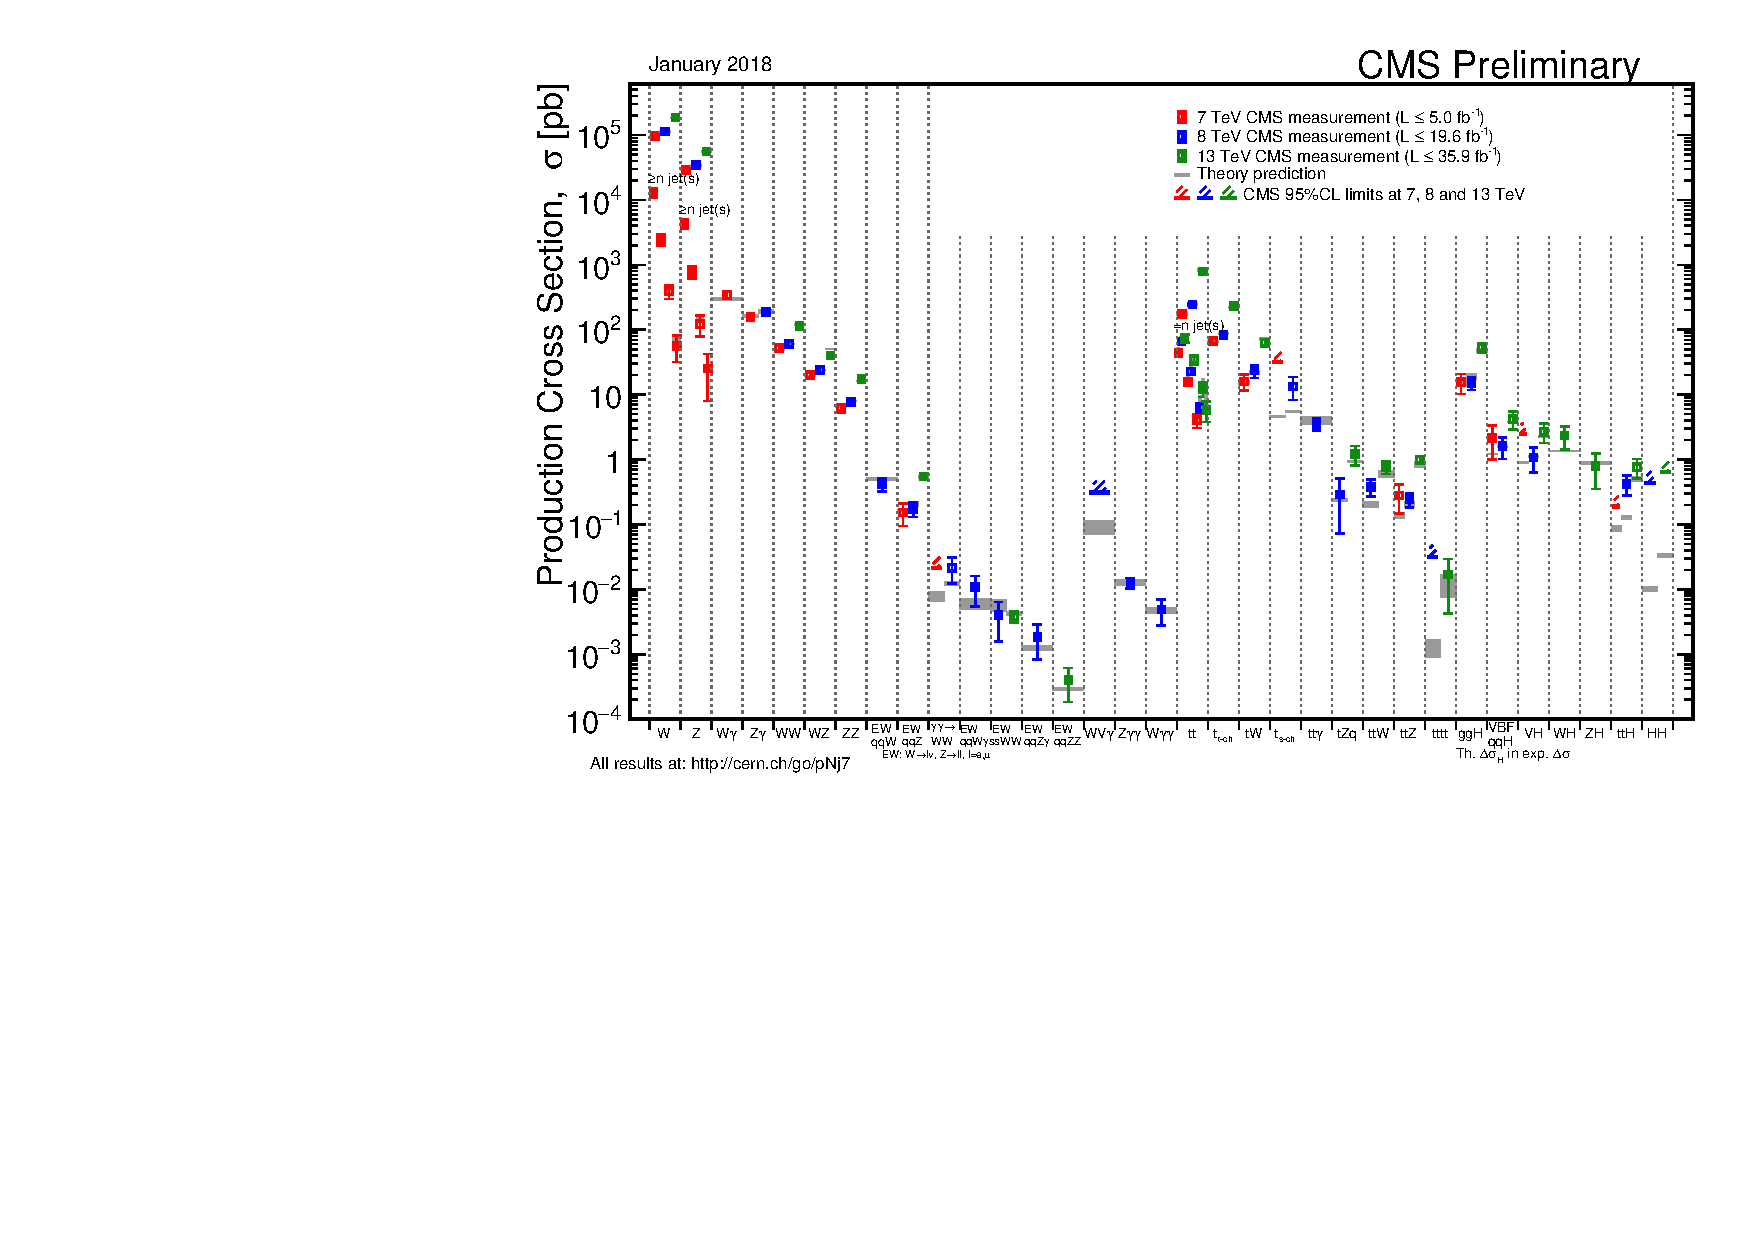
\includegraphics[width=0.95\textwidth]{plot/SigmaNew_v0.pdf}
	\label{fig1-1}
	\caption{Compilation of different SM predictions compared to the corresponding CMS cross section measurements.}
	\end{figure*}
	
\FloatBarrier
\section{Problems of the Standard Model}
Although the SM is remarkably successful at explaining a wide range of phenomena, it does leave many questions unanswered. 
One major problem is the omission of the gravity - the most familiar fundamental force. 
Phenomena at large scale can be well described by the general relativity, however, there is not yet a satisfactory theory which can incorporate the gravity at subatomic scale. 
Therefore the SM is believed to be a low-energy approximation of a theory existing at the $10^{19}$ GeV Planck scale ($M_{Pl}$), the energy at which the gravity is comparable to the other forces and can no longer be ignored.

Another outstanding problem of the SM is the lack of explanation for dark matter (DM), so named because it doesn't undergo electromagnetic interactions and thus is invisible to normal matter. The dark matter was discovered through the measurement of velocity dispersion and rotation curves of the galaxies, whose results indicated that the luminous matter cannot explain the observed curves on its own and some invisible matter is needed to account for. Measurements show that roughly 80\% of the matter in the universe is made of dark matter. Despite the extensive experimental efforts of searching for the DM, we still know little about the nature of the DM and its interactions with the normal matter described by the SM. 

Besides the lack of particle candidates for the gravity and DM, there are some observations that the SM  cannot explain. 
One of these mysteries is the large discrepancy between the electroweak and Planck scale, which is known as the hierarchy problem. 
The Higgs mass is measured to be 126 GeV, $10^{17}$ lower than the Planck scale. 
The physical mass of the Higgs is a combination of the tree-level bare mass and high order corrections. 
Because the loop corrections of the Higgs mass contains quadratic divergences, its bare mass has to cancel the corrections with an accuracy up to 34 digits leaving a small mass at electroweak scale. 
This unnatural cancellation is called ``fine tuning problem'', and it suggests the appearance of new physics which can stabilize the Higgs mass.

Due to these issues, the SM is considered as an incomplete theory.
Many new theories beyond the SM have been introduced to incorporate the unexplained features in the SM. 
Some of the popular extensions of the SM include supersymmetry models, composite Higgs models and large extra dimensions.
We will in this thesis focus on the supersymmetric extension of the SM.    


\section{Supersymmetry}

Supersymmetry (SUSY) is a favored extension of the SM that provides solutions for many of the problems of the SM. 
It unifies the description of forces and matter by inducing a symmetric transformation between bosons and fermions. 
The supersymmetry transformations are generated by operator $\OpQ$, which is called the supercharge. 
The operator $\OpQ$ acts on the states, turning a fermionic component into a bosonic component, and vice verse, as: 
      \begin{equation}
        \OpQ \ket{ \text{Boson} } = \ket{ \text{Fermion}},   \quad   \OpQ \ket{\text{Fermion}} = \ket{ \text{Boson}}.
      \end{equation} 

The supercharge itself is a spinor, so its hermitian conjugate $\OpQ^\dagger$ is also a symmetry generator. 
They satisfy the following anti-commutation relations:
    \begin{equation}
     \{\OpQ_a, \OpQ_{\dot{a}}^\dagger \} = (\sigma^\mu})_{a\dot{a}} P_\mu,
      \label{eqn:commutation}
     \end{equation} 
    \begin{equation}
     \{\OpQ_a, \OpQ_b \} = 0, \quad
     \{\OpQ_{\dot{a}}^\dagger, \OpQ_{\dot{b}}^\dagger \} = 0,
      \end{equation} 
      \begin{equation}
     [\OpQ_a, P_\mu] = 0, \quad  [\OpQ_{\dot{a}}^\dagger,  P_\mu] = 0.
    \end{equation} 
where $P_\mu = i\partial_\mu$ is the momentum operator. 
The first anti-commutation relation, equation \ref{eqn:commutation}, indicates that the product of two supersymmetric transformations results in translations in space-time.

\subsection{The Minimal Supersymmetric Standard Model }
SUSY doubles the number of particles by paring each particle with a SUSY partner - each fermion has a bosonic partner and each gauge boson has a fermionic partner. 
The particle and its superpartner has the same quantum number except the spin. The SM fields and superpartiners are grouped together into supermultiplets. 
With this general concept of SUSY, one can build models with any number of supermultiplets. 
To solve the hierarchy problem, it is appropriate to first consider the simplest version of the SUSY models, which contains the minimum number of SUSY particles and new interactions. 
Such a model is referred to as the Minimal Supersymmetric Standard Model (MSSM). 

In MSSM, all the SM fermions are taken to be the fermonic components of chiral supermultiplets. 
Each of them is paired with a spin 0 scalar partner, whose name is obtained by adding a prefix $s$ to the name of the corresponding SM particle.
For example, the scalar partner of an electron is called selectron, and the scalar quarks are called squark. 
The SM gauge fields are taken to be the members of vector supermultiplets and are paired with spin $1/2$ superpartners. 
The naming convention for the spin $1/2$ superpartners is to add $-ino$ after the name of the SM gauge bosons. 
So for $B$, $W^{\pm, 0}$ and gluons, the superpartners are Bino, Winos and gluinos. 
Different with the SM, in MSSM two Higgs doublets are required to break the electroweak symmetry. 
The scalar Higgs fields are paired with spin $1/2$ partners, which are named Higgsinos, to form the chiral multiplets.
Table \ref{tab:MSSM} lists the particle content of the MSSM. 

\begin{table}[hbtp]
\centering
\begin{tabular}{ |c|c|c|c|c|}
	\hline \hline
	\multicolumn{5}{ |c| }{ MSSM particles } \\
	\hline
	 	 &  \multicolumn{2}{|c|}{SUSY particle fields} & \multicolumn{2}{ |c| }{Particle fields}  \\
	\cline{2-5}
		 &  name & symbol & name &symbol  \\
	\hline
	\multirow{5}{*}{sfermion/femion} & \multirow{2}{*}{slepton} & $(\tilde{\nu}_l, \tilde{l})_L$ & \multirow{2}{*}{lepton} & $(\nu_l, l)_L$ \\
	                                                    &                                      &  $\tilde{l}_R$                      &                                     &  $l_R$ \\
	\cline{2-5}
	                                                    & \multirow{3}{*}{squark} & $(\tilde{u}, \tilde{d})_L$      & \multirow{3}{*}{quark}      & $(u,d)_L$ \\
	                                                    &                                      &  $\tilde{u}_R$                      &                                     &  $u_R$ \\
	                                                 	  &                                      &  $\tilde{d}_R$                      &                                     &  $d_R$ \\
	\hline
	\multirow{3}{*}{gaugino/gauge boson} & Bino                     & $\tilde{B}$                           & B boson                      & $B$ \\
	\cline{2-5}                                                           
	                                                            &  Wino                   & $\tilde{W}^\pm$, $\tilde{W}^0$  & W boson               & $W^\pm$, $W^0$ \\
	\cline{2-5}                                                           
	                                                            &  Gluino                   & $\tilde{g}$                         & Gluon                          & $G$ \\
	\hline
	\multirow{2}{*}{higgsino/higgs}    & \multirow{2}{*}{higgsino} & $(\tilde{H}_d^0, \tilde{H}_d^-)$  & \multirow{2}{*}{higgs} &  $(H_d^0, H_d^-)$\\
	                                                    &                                         &  $(\tilde{H}_u^+, \tilde{H}_u^0)$ &                            &  $(H_u^+, H_u^0)$\\                                                      

	\hline	                                     		 
\end{tabular}
\label{tab:MSSM} 
\end{table}

Constructing a supersymmetric Lagrangian in the 4-dimensional spacetime can be very difficult and tedious. 
The introduction of superspace greatly simplified the calculations. 
The superspace extends the usual spacetime coordinates with two fermionic (or Grassmannian) coordinates. 
Points in superspace have coordinates:
     \begin{equation}
	(x^\mu, \theta, \theta^\dagger)
     \end{equation}
where $x^\mu$ are space-time coordinates and $\theta$, $\theta^\dagger$ are anti-commuting Grassmann variables.
Supermultiplets are described by functions over the superspace, which are referred to as superfield. 
A chiral superfield can be expressed by expansion in Grassmann variables as:
    \begin{equation}
    \Phi(x, \theta, \theta^\dagger) = \phi(x) + \theta\psi(x) + \frac{1}{2}\theta\theta F(x) + (\text{space-time derivatives acting on}\ \phi \ {and}\  \psi)
    \end{equation}
 where $\phi$ is a complex scalar field, $\psi$ is a left-chiral spinor, and $F(x)$ is an auxiliary field. 
 The auxiliary field is introduced to ensure that the number of bosonic and fermionic degrees of freedom match with each other for both on-shell and off-shell cases. 
 
 A general vector superfield fixed by the Wess-Zumino gauge can be expressed as: 
 	\begin{equation}
		V = -\theta \sigma^\mu \bar{\sigma}V_\mu{x} + i\theta^2 \bar{\theta}\bar{\lambda}(x) -  i\bar{\theta}^2 \theta\lambda(x) + \frac{1}{2}\theta^2 \bar{\theta}^2 D(x).
	\end{equation}
Here the $V_\mu(x)$ is the gauge field, $\lambda(x)$ and $\bar{\lambda}(x)$ are gauginos, and $D(x)$ is the auxiliary field. 

Then the supersymmetric Lagrangian can be conveniently written as: 
	\begin{equation}
		\mathcal{L} = \int d^4\theta \Phi_i^\dagger e^{gV}\Phi_i + \int d^2\theta (\frac{1}{4}W_\alpha^a W^{\alpha a} + h.c.) + \int d^2\theta (W(\Phi) + h.c.)
		 \label{eq:SUSYL}
	\end{equation}
where $W(\Phi)$ is the super potential of the chiral fields. The superpotential of the MSSM has the form: 
	\begin{equation}
		W = 	l^i\Phi_i + \frac{1}{2}m^{ij} \Phi_i \Phi_j + \frac{1}{6} y^{ijk} \Phi_i \Phi_j \Phi_k.
	\end{equation}
	
The $W^{\alpha a}$ in \ref{eq:SUSYL} is the field-strength of the vector superfile,
	\begin{equation}
		W_\alpha = - \frac{1}{4}\bar{D}^\alpha \bar{D}_\alpha D_\alpha V
	\end{equation}
where $D_\alpha$ is the covariant derivatives in superspace. 

SUSY provides a solution to the hierarchy problem. 
In the loop corrections to the Higgs self energy, the contributions from fermions and bosons cancel with each other, leaving a light Higgs mass at the electroweak scale. This is illustrated in Fig. \ref{fig:susyhiggs}. \\

\begin{figure*}[hbtp]
\centering
\begin{fmffile}{simple_tree}
\begin{fmfgraph*}(150,70)
\fmfleft{i}
\fmfright{o}
\fmflabel{$h$}{i}
\fmflabel{$h$}{o}
\fmf{dashes}{i,v1}
\fmf{dashes}{v2,o}
\fmf{fermion,label=$t$,left,tension=0.4}{v1,v2,v1}
\end{fmfgraph*}
\end{fmffile}  \quad \quad 
\begin{fmffile}{simple_susy}
\begin{fmfgraph*}(150,70)
       \fmfleft{i}
       \fmfright{o}
       \fmftop{m}
       \fmfv{label=h,l.a=60}{i}
       \fmfv{label=h,l.a=120}{o}
       \fmflabel{$\widetilde{\text{t}}$}{m}
       \fmf{dashes,tension=1}{i,v1}
       \fmf{dashes,tension=1}{v1,o}
       \fmf{dashes,right,tension=0}{v1,m,v1}
    \end{fmfgraph*}}
%\fmfleft{i}
%\fmfright{o}
%\fmflabel{$h$}{i}
%\fmflabel{$h$}{o}
%\fmf{dashes}{i,v1}
%\fmf{dashes}{v1,o}
%\fmf{fermion,label=$\tilde{t}$,left,tension=0.4}{v1,v1}
%\end{fmfgraph*}
\end{fmffile}  \\
\bigskip
\label{fig:susyhiggs}
\caption{Contributions of SM and SUSY loop corrections to the mass of Higgs.} 
\end{figure*}\\

SUSY also provides candidate for the dark matter.  If R-parity is conserved, the lightest SUSY particle (LSP) is stable. It can serve as an dark matter candidate. 
For DM which are weakly interacting massive particles (WIMPs), the interactions between the DM and normal particles are so weak that the DM will escape the detector, resulting in momentum imbalance in the transverse plane.
This signature allows the searches for SUSY in the particle colliders. 


\subsection{Supersymmetry Breaking}
As mentioned before, the quadratic divergence of the Higgs mass arising from SM loop can be exactly cancelled by the contribution from SUSY partners when the masses of all states in a supermultiplet are degenerate. 
However, any partners with the same mass of leptons or light quarks should have been observed. 
Therefore supersymmetry must be a broken symmetry at low energy scale if it is realized in nature. 
In order to maintain the good ultraviolet behaviour of the supersymmetry while split the mass between the SM particles and their SUSY partners, a soft symmetry breaking is considered. 
The idea is that supersymmetry is unbroken at some high energy scale at which the exact SUSY is preserved. 
At low energy scale, the supersymmetry breaking takes place, allowing the SUSY particles to obtain heavier mass than their SM partners.
This can be achieved by introducing soft breaking terms into the Lagrangian. The MSSM soft-breaking terms are:
	\begin{equation}
	\begin{array}{c l l }
		\mathcal{L}_{soft} &=& - \frac{1}{2} ( M_1 \tilde{B} \tilde{B} + M_2 \tilde{W} \tilde{W} + M_3 \tilde{g} \tilde{g} ) \\
					  & & - (a_u\tilde{Q}H_u\tilde{\bar{u}} + a_d\tilde{Q}H_d\tilde{\bar{d}} +  a_e\tilde{L}H_e\tilde{\bar{d}} ) \\
					  & & - m_{H_u}^2 |H_u|^2 - m_{H_d}^2 |H_d|^2 - bH_uH_d \\
			 &  &  - M_Q^2 |\tilde{q}_L |^2 - M_U^2 |\tilde{u}_R |^2  - M_D^2 |\tilde{u}_D |^2 - M_L^2 |\tilde{l}_L |^2 - M_E^2 |\tilde{l}_R |^2.
	\end{aligned}
	\end{equation}      
The coefficient of each term is called soft SUSY breaking parameter. 
The appearance of the soft breaking terms introduces 105 more independent parameters. 
Assuming these breaking terms originate from the same mechanism, the scale of the SUSY breaking can be denoted as $m_{\text{SUSY}}$:
	\begin{equation}
		\begin{array}{c c c}
			M_{1,2,3}, a_{u,d,e} & \sim & m_{\text{SUSY}} \\
			M^2_{Q,U,D,L,E,H_u, H_d}, b & \sim & m^2_{\text{SUSY}}
		\end{array}
	\end{equation}

To understand the origin of these breaking terms, we can consider the soft supersymmetry breaking as an effective description of  the spontaneous supersymmetry breaking, i.e. the Lagrangian is invariant under supersymmetric transformations but the vacuum state is not. 
The spontaneous supersymmetry breaking happens when the supercharges do not annihilate the vacuum, i.e., 
    \begin{equation}
	\OpQ \ket{0} \neq 0
    \end{equation}
Using the commutation relation \label{eq:commutation} of the supercharges, we can write the Hamiltonian as
	 \begin{equation}
		H = P^0 = \frac{1}{4}(\OpQ_1\bar{\OpQ}_\dot{1}} + \bar{\OpQ}_{\dot{1}} \OpQ_1 + \OpQ_2 \bar{\OpQ}_{\dot{2}} + \bar{\OpQ}_{\dot{2}}  \OpQ_2 )
	  \end{equation}
which has positive vacuum expectation value (VEV) when SUSY is spontaneous broken, i.e.
	 \begin{equation}
	\langle 0| H |0 \rangle  > 0.
	\end{equation}

SUSY breaking within the MSSM is not easy, because it predicts SUSY particles that are lighter than their SM partners. 
The way out is to assume the existence of a hidden sector that is uncharged under the SM gauge group. 
The SUSY breaking originates in the hidden sector and communicate to the visible MSSM sector by a set of messenger fields. 
The messenger sector transmits the SUSY breaking via loop corrections, allowing the SUSY particles to become massive. 
There are several well studied mechanism for mediating the SUSY breaking to the visible sector, including gravity mediation, gauge mediation and anomaly mediation. 
The search presented in this thesis is motivated by the gauge mediated SUSY breaking (GMSB). 

The GMSB mechanism assume that the messenger sector couple to the visible sector via flavor-blind gauge interactions. 
Suppose the hidden sector has some supermultiplet S which has VEV $\langle F \rangle$, where F is the auxiliary field of S. 
A set of messenger fields ${\Phi_I, \bar{\Phi}_I}$ couple to the hidden sector via interaction term:
	 \begin{equation}
	W = \sum_I y_I S \Phi_I \bar{\Phi}_I.
	\end{equation}
If $\langle F \rangle$ is non-zero, mass splittings are generated in the messenger sector. 
The messenger fields are charged under the SM gauge. 
Therefore the SUSY breaking is mediated from the hidden sector to the visible sector through gauge interaction. A scheme of the gauge mediation is shown in Figure \ref{fig:GMSB}. 

	\begin{figure*}[!h]
		\centering
		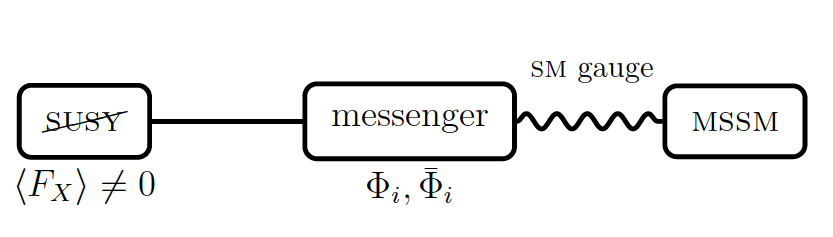
\includegraphics[width=0.6\textwidth]{plot/GMSB.png}
		\caption{SUSY breaking in the hidden sector is mediated to the MSSM sector via the messenger fields.}
		\label{fig:GMSB}
	\end{figure*}

The gauginos become heavier due to the radiative corrections from messenger particle loops, as illustrated in the Feynman diagram of Figure \ref{fig:messanger}. 

\begin{figure*}[!h]
	\centering
		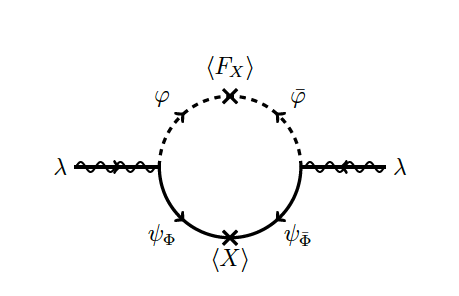
\includegraphics[width=0.4\textwidth]{plot/mess.png}
	\caption{Radiative corrections to the mass of SUSY particles.}
	\label{fig:messanger}
\end{figure*}

Assuming that the messenger fields have mass $M_{mess}$, we can integrate out the messenger fields to get the effective SUSY breaking. 
The resulting soft mass is proportional to
	\begin{equation}
		M_{soft} \sim \frac{ \langle F \rangle}{M_{mess}}
	\end{equation}
If the $M_{mess}$ and $\sqrt{\langle F \rangle}$ are of the same order, the SUSY breaking can be realized in a scale as low as the electroweak scale. 
Requiring the gravity effects to be negligible, one can also impose an $10^{15}$ GeV upper bound on the scale of $M_{mess}$. \\

When the electroweak symmetry is broken, only the SU(3) and U(1) gauge remains unbroken. 
Similar to the mixing of the gauge bosons in the SM, the Bino, Winos and higgsinos will mix to form mass eigenstates.
The mixing of two neutral gauginos ($\widetilde{B}, \widetilde{W}^0$) and two neutral higgsinos ($\widetilde{h}_d^0, \widetilde{h}_u^0$) will give rise to four neutral mass eigenstates called neutralinos, denoted as $\widetilde{\chi}^0_{1,2,3,4}$. The mixing mass matrix for the neutralinos is: 
	\begin{equation}
		 M_N  = \left(
			 \begin{array}{c c c c }
			 	 M_1                           & 0                                & -M_Z cos\beta S_W & M_Z cos\beta S_W  \\
				   0                                & M_2                          & M_Zcos\beta C_W   & -M_Zsin\beta C_W  \\
				 -M_Z cos\beta C_W  & M_Z sin\beta C_W   & 0                                &  \mu \\
				 M_Z sin\beta S_W     & -M_Z cos\beta S_W  & \mu                          &  0
			\end{array}
		\right)
	\end{equation}
Similarly, the charged gaugino-higgsino mixing will give rise to four charged mass eigenstates.
The mixing matrix is: 
	\begin{equation}
		M_C = \left(
			\begin{array}{c c }
				M_2            & \sqrt{2}M_W sin\beta \\
				\sqrt{2}M_W cos\beta     &  \mu   
			\end{array}
		\right)
	\end{equation}
The resulting mass eigenstates, $\widetilde{\chi}^\pm_1, \widetilde{\chi}^\pm_2$, are called the charginos.

\subsection{Phenomenology of General Gauge mediation Supersymmetry}

According to the Goldstone's theorem, for every global symmetry with spontaneous breaking there exist a massless Nambu-Goldstone boson. 
Similar to the goldstone boson, spontaneous SUSY breaking gives rise to a massless goldstino. 
When SUSY is imposed as a local symmetry, the goldstino is absorbed by the gravitino, becoming the longitudinal component of the gravitino. 
The gravitino mass scales as:
	\begin{equation}
		m_{2/3} \sim \langle F \rangle/M_{PL}
	\end{equation}
The SUSY breaking scale could be very low in gauge-mediated models, making the gravitino to have a mass roughly in the 1 eV to 1 GeV range.  
Therefore, one important consequence of the GMSB is that gravitino is the lightest supersymmetry particle (LSP).
All the heavier SUSY particles will eventually decay to the graviton, either directly or through a cascade decay chain. 
Therefore, the phenomenology is mainly determined by the nature of the next-to-lightest SUSY particle (NLSP).\\

The decay length of the NLSP is promotional to $\langle F \rangle^2$. 
Depending on the scale of the messenger mass, the decay of the NLSP can be prompt, long-lived or outside the detector. 
In this search, we will focus on the prompt scenarios: the NLSP immediately decay to its SM partner and a gravitino. 
In the general gauge-mediated (GGM) models, the NLSP could be the lightest neutralino. 
The general neutralino NLSP senarios lead to very interesting signatures involving photons, $W$, $Z$ or higgs in the final states. \\

The neutralino NLSP is a mixture of the neutral gauginos and higgsinos. 
Depending on the relative hierarchy among the soft masses, the NLSP can be one of the three cases:
\begin{itemize}
	\item Bino-Like: if $|M_1| < |\mu|,|M_2|$, the neutralino NLSP is mostly a Bino. It will dominantly decay through the $\tilde{\chi}_1^0 \rightarrow \gamma + \tilde{G}$ channel. 
	         The typical signature of Bino-like neutralino pair production is large transverse missing momentum plus a pair of photons in the final states.  
	\item Wino-like: if $|M_2| < |\mu|, |M_1|$, the neutralino NLSP is dominated by the Wino component. 
		Since the wino multiplet consists of both charged ($\tilde{W}^\pm$) and neutral ($\tilde{W}^0$) gauginos, the lightest chargino ($\tilde{\chi}_1^\pm$) can be as light as the neutralino NLSP. 
		In this case, the $\tilde{\chi}_1^0$ and $\tilde{\chi}_1^\pm$ are nearly mass degenerate, and they are called the co-NLSP. 
		The wino-like $\tilde{\chi}_1^0$ can decay into $\gamma + \tilde{G}$ or $Z + \tilde{G}$. 
		The branching fraction of the wino-like $\tilde{\chi}_1^0$ decay is shown in Figure \ref{fig: neuBR}. 
		On the other hand, the $\tilde{\chi}_1^\pm$ decays to the $W^\pm+ \tilde{G}$ final states, where the $W$ boson can decay hadroniclly or leptonically. 
		Depending on the decay mode of the NLSP and the $W/Z$ bosons, the final states can contain photons or leptons plus large transverse momentum. 
	\item Higgsino-like: if $\mu < |M_1|, |M_2|$, the NLSP is higgsino-like. The decay mode of the NLSP varies with the mass parameters and mixing angles. In the case where the $h + \tilde{G}$ decay mode is preferred, one can use events containing higgs to probe the production of higgsino-like NLSP and enhance the search sensitivity. 
\end{itemize}

In this thesis we present a search for GGM SUSY signatures involving the production of wino-like $\tilde{\chi}_1^0\tilde{\chi}_1^\pm$ pairs in final states with a photon, a lepton (either $e$ or $\mu$) and significant missing momentum. 
Photons (leptons) in the final state are the result of neutralino (chargino) decays to a gravitino and a photon (W boson), $\tilde{\chi}_1^0 \rightarrow \gamma + \tilde{G}$ ( $\tilde{\chi}_1^\pm \rightarrow W^\pm+ \tilde{G}$, with $W^\pm \rightarrow l + \nu$).
The additional lepton in the final state not only suppresses the backgrounds from QCD processes, but also offers the unique opportunity to probe the branching fractions of the NLSP.  

\subsection{Simplified Models of Supersymmetry}

There are many different manifestations of SUSY, each with different particle contents and mechanisms for SUSY breaking. 
However, many of these models predict a similar phenomenology, which inspired the formulation of the simplified models.
The simplified models use effective Lagrangian to describe the new particles and their decays. 
The masses of the particles and the branching ratio of their decays can be tuned directly. 

In this analysis we consider both the simplified models and GGM senarios to interpret the search results. 
Here only the productions of a pair of primary particles are considered. 
Figure \ref{fig:crosssection} shows the cross sections of the production of $\tilde{g}\tilde{g}$, $\tilde{q}\tilde{\bar{q}}$ and $\tilde{\chi}_1^0\tilde{\chi}_1^\pm$ pairs as a function of the primary particle mass. 
Each primary particle undergos a direct decay or a cascade decay through an SUSY particle and ends with the LSP. 

	\begin{figure*}[!h]
		\centering
		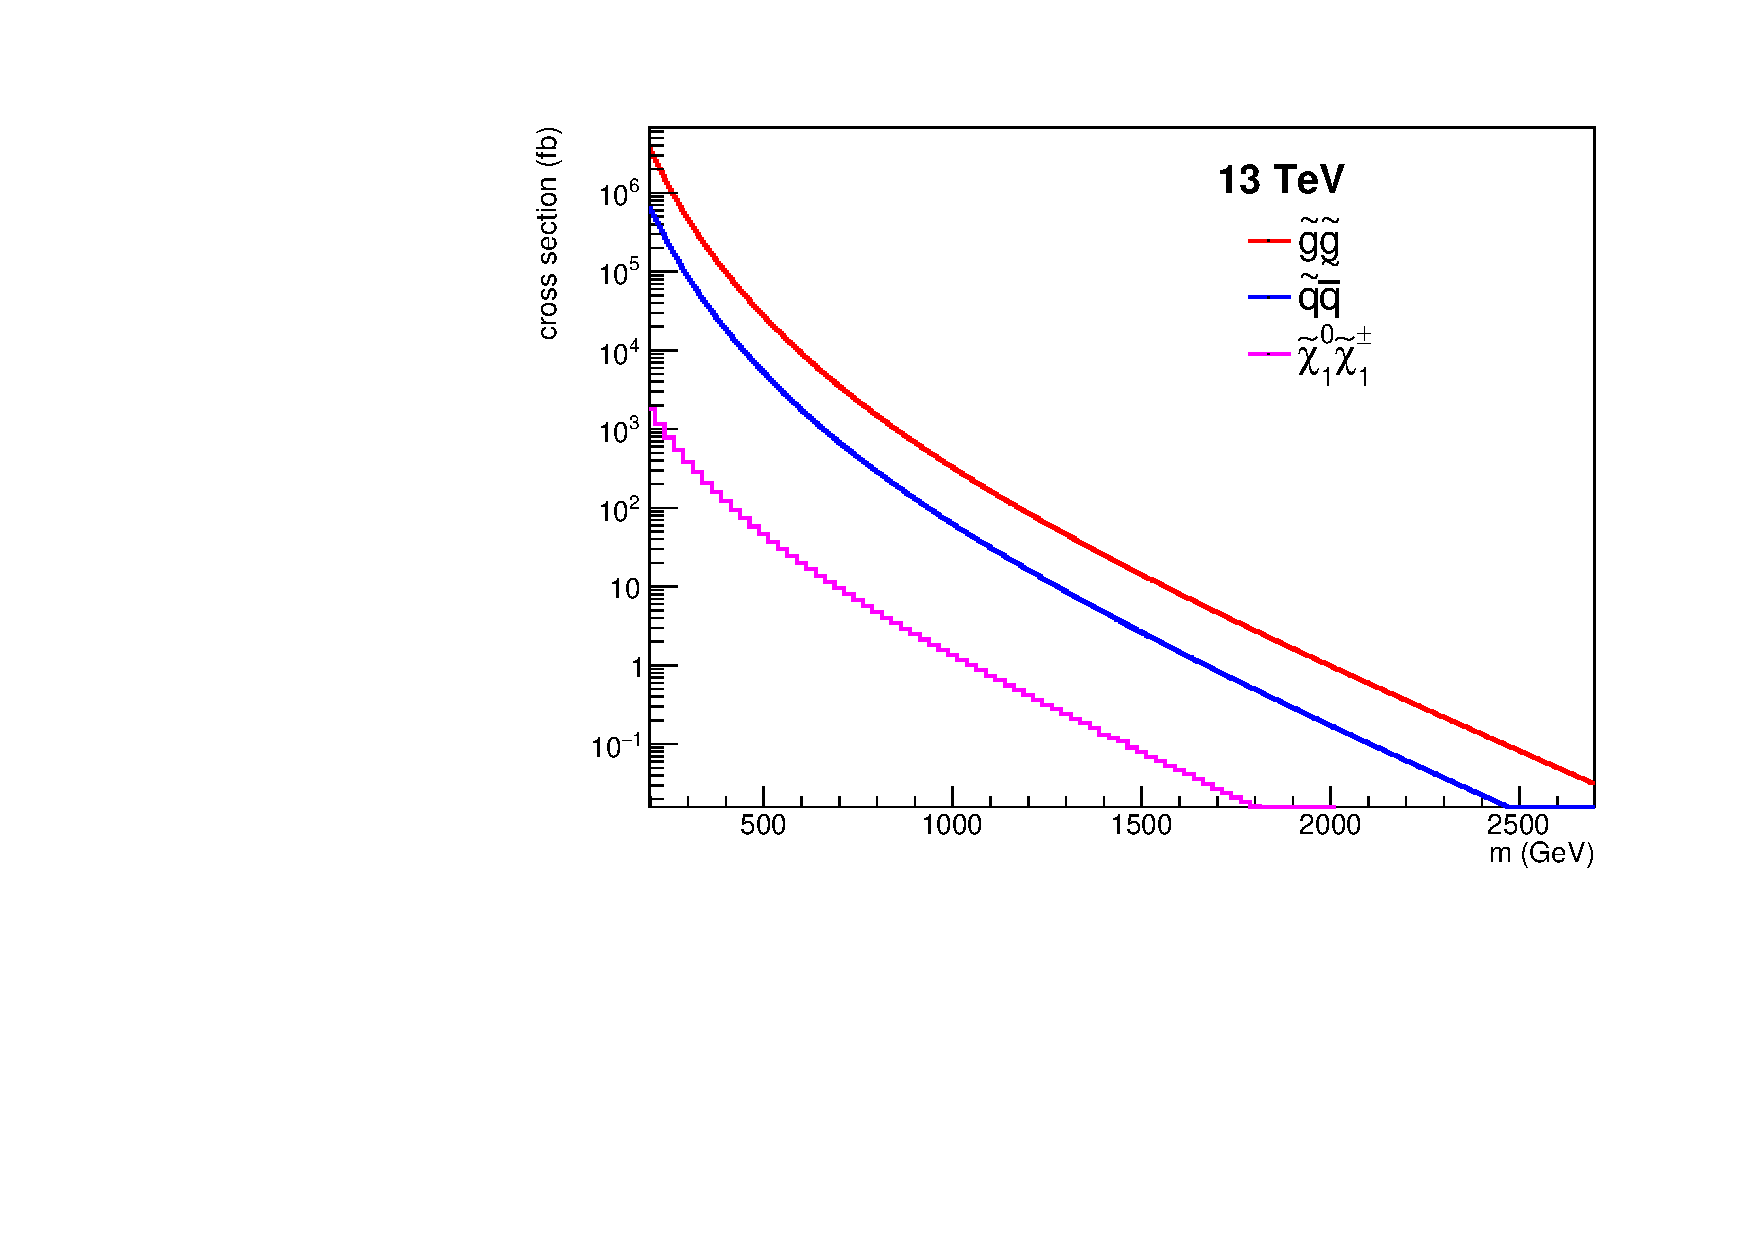
\includegraphics[width=0.5\textwidth]{plot/xs_thesis.pdf}
		\caption{Cross sections for producing various pairs of sparticles at $\sqrt{s} =$ 13 TeV.} 
		\label{fig:crosssection}
	\end{figure*}

The simplified models considered in this analysis include the following three processes: 
	\begin{itemize}
		\item \textbf{TChiWG}: This model assumes the direct production of $\tilde{\chi}_1^0/\tilde{\chi}_1^\pm$ pairs. The $\tilde{\chi}_1^0$ and $\tilde{\chi}_1^\pm$ are taken to be mass degenerate. The $\tilde{\chi}_1^0$ undergos direct decay to a photon and LSP, while the $\tilde{\chi}_1^\pm$ decays to $W^\pm$ plus LSP. 
		\item  \textbf{T5WG}: This model is a simplified version of gluino pair production in which each gluino decays to a quark-antiquark pair and intermediate neutralino or chargino. The mass of the neutralino and chargino are set to be the same. A 50\% branching ratio is assumed for the gluino to neutralino/chargino decay. 
		\item \textbf{T6WG}: Similar to the T5WG model, productions of a pair of squarks are assumed in the T6WG model. The squark decays to an SM quark plus an intermediate neutralino or chargino. The branching ratio for the squark to neutralino/chargino is also assumed to be 50\%. 
	\end{itemize}
These processes are illustrated in the Feynman diagrams in Figure \ref{fig:feyngmsb}.

	\begin{figure*}[!h]
	\centering
		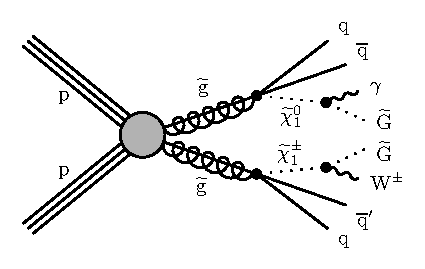
\includegraphics[width=0.4\textwidth]{plot/gitT5qqqqWG.pdf}
		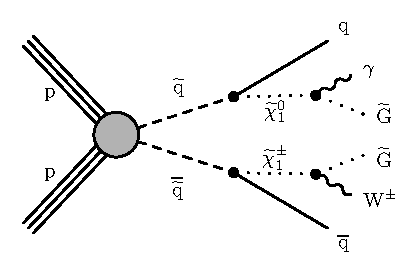
\includegraphics[width=0.4\textwidth]{plot/gitT6qqWG.pdf}  \\
		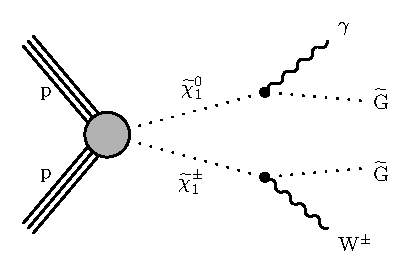
\includegraphics[width=0.4\textwidth]{plot/gitTChiGW.pdf} 
	\caption{Feynman diagrams showing the production and decay modes of the signal models T5Wg (top left), T6Wg (top right), and TChiWg (bottom) considered in this analysis.}
	\label{fig:feyngmsb}
	\end{figure*}



\end{document}


